% Created by tikzDevice version 0.12.4 on 2023-06-03 16:04:22
% !TEX encoding = UTF-8 Unicode
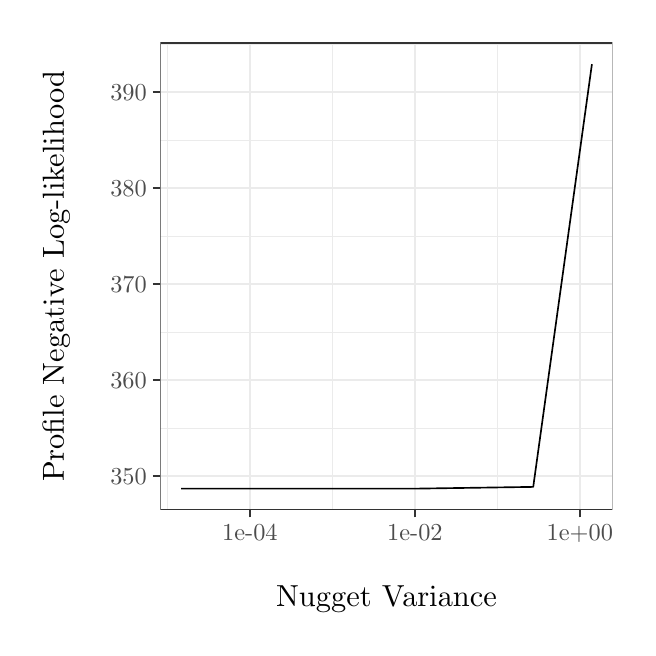
\begin{tikzpicture}[x=1pt,y=1pt]
\definecolor{fillColor}{RGB}{255,255,255}
\path[use as bounding box,fill=fillColor,fill opacity=0.00] (0,0) rectangle (216.81,216.81);
\begin{scope}
\path[clip] (  0.00,  0.00) rectangle (216.81,216.81);
\definecolor{drawColor}{RGB}{255,255,255}
\definecolor{fillColor}{RGB}{255,255,255}

\path[draw=drawColor,line width= 0.6pt,line join=round,line cap=round,fill=fillColor] (  0.00,  0.00) rectangle (216.81,216.81);
\end{scope}
\begin{scope}
\path[clip] ( 47.99, 42.57) rectangle (211.31,211.31);
\definecolor{fillColor}{RGB}{255,255,255}

\path[fill=fillColor] ( 47.99, 42.57) rectangle (211.31,211.31);
\definecolor{drawColor}{gray}{0.92}

\path[draw=drawColor,line width= 0.3pt,line join=round] ( 47.99, 72.15) --
	(211.31, 72.15);

\path[draw=drawColor,line width= 0.3pt,line join=round] ( 47.99,106.82) --
	(211.31,106.82);

\path[draw=drawColor,line width= 0.3pt,line join=round] ( 47.99,141.48) --
	(211.31,141.48);

\path[draw=drawColor,line width= 0.3pt,line join=round] ( 47.99,176.15) --
	(211.31,176.15);

\path[draw=drawColor,line width= 0.3pt,line join=round] ( 47.99,210.82) --
	(211.31,210.82);

\path[draw=drawColor,line width= 0.3pt,line join=round] ( 50.49, 42.57) --
	( 50.49,211.31);

\path[draw=drawColor,line width= 0.3pt,line join=round] (110.11, 42.57) --
	(110.11,211.31);

\path[draw=drawColor,line width= 0.3pt,line join=round] (169.73, 42.57) --
	(169.73,211.31);

\path[draw=drawColor,line width= 0.6pt,line join=round] ( 47.99, 54.82) --
	(211.31, 54.82);

\path[draw=drawColor,line width= 0.6pt,line join=round] ( 47.99, 89.48) --
	(211.31, 89.48);

\path[draw=drawColor,line width= 0.6pt,line join=round] ( 47.99,124.15) --
	(211.31,124.15);

\path[draw=drawColor,line width= 0.6pt,line join=round] ( 47.99,158.82) --
	(211.31,158.82);

\path[draw=drawColor,line width= 0.6pt,line join=round] ( 47.99,193.48) --
	(211.31,193.48);

\path[draw=drawColor,line width= 0.6pt,line join=round] ( 80.30, 42.57) --
	( 80.30,211.31);

\path[draw=drawColor,line width= 0.6pt,line join=round] (139.92, 42.57) --
	(139.92,211.31);

\path[draw=drawColor,line width= 0.6pt,line join=round] (199.53, 42.57) --
	(199.53,211.31);
\definecolor{drawColor}{RGB}{0,0,0}

\path[draw=drawColor,line width= 0.6pt,line join=round] ( 55.41, 50.24) --
	( 76.63, 50.24) --
	( 87.23, 50.24) --
	( 92.53, 50.24) --
	( 95.18, 50.24) --
	( 96.51, 50.24) --
	( 97.17, 50.24) --
	( 97.50, 50.24) --
	( 97.67, 50.24) --
	( 97.75, 50.24) --
	( 97.79, 50.24) --
	( 97.82, 50.24) --
	( 97.83, 50.24) --
	( 97.83, 50.24) --
	( 97.83, 50.24) --
	( 97.83, 50.24) --
	( 97.83, 50.24) --
	( 97.84, 50.24) --
	( 97.84, 50.24) --
	( 97.84, 50.24) --
	( 97.85, 50.24) --
	( 97.87, 50.24) --
	( 97.92, 50.24) --
	( 98.00, 50.24) --
	( 98.16, 50.24) --
	( 98.50, 50.24) --
	( 99.16, 50.24) --
	(100.48, 50.24) --
	(103.14, 50.24) --
	(108.44, 50.24) --
	(119.04, 50.24) --
	(140.25, 50.24) --
	(182.68, 50.87) --
	(203.89,203.64);
\definecolor{drawColor}{gray}{0.20}

\path[draw=drawColor,line width= 0.6pt,line join=round,line cap=round] ( 47.99, 42.57) rectangle (211.31,211.31);
\end{scope}
\begin{scope}
\path[clip] (  0.00,  0.00) rectangle (216.81,216.81);
\definecolor{drawColor}{gray}{0.30}

\node[text=drawColor,anchor=base east,inner sep=0pt, outer sep=0pt, scale=  0.88] at ( 43.04, 51.79) {350};

\node[text=drawColor,anchor=base east,inner sep=0pt, outer sep=0pt, scale=  0.88] at ( 43.04, 86.45) {360};

\node[text=drawColor,anchor=base east,inner sep=0pt, outer sep=0pt, scale=  0.88] at ( 43.04,121.12) {370};

\node[text=drawColor,anchor=base east,inner sep=0pt, outer sep=0pt, scale=  0.88] at ( 43.04,155.79) {380};

\node[text=drawColor,anchor=base east,inner sep=0pt, outer sep=0pt, scale=  0.88] at ( 43.04,190.45) {390};
\end{scope}
\begin{scope}
\path[clip] (  0.00,  0.00) rectangle (216.81,216.81);
\definecolor{drawColor}{gray}{0.20}

\path[draw=drawColor,line width= 0.6pt,line join=round] ( 45.24, 54.82) --
	( 47.99, 54.82);

\path[draw=drawColor,line width= 0.6pt,line join=round] ( 45.24, 89.48) --
	( 47.99, 89.48);

\path[draw=drawColor,line width= 0.6pt,line join=round] ( 45.24,124.15) --
	( 47.99,124.15);

\path[draw=drawColor,line width= 0.6pt,line join=round] ( 45.24,158.82) --
	( 47.99,158.82);

\path[draw=drawColor,line width= 0.6pt,line join=round] ( 45.24,193.48) --
	( 47.99,193.48);
\end{scope}
\begin{scope}
\path[clip] (  0.00,  0.00) rectangle (216.81,216.81);
\definecolor{drawColor}{gray}{0.20}

\path[draw=drawColor,line width= 0.6pt,line join=round] ( 80.30, 39.82) --
	( 80.30, 42.57);

\path[draw=drawColor,line width= 0.6pt,line join=round] (139.92, 39.82) --
	(139.92, 42.57);

\path[draw=drawColor,line width= 0.6pt,line join=round] (199.53, 39.82) --
	(199.53, 42.57);
\end{scope}
\begin{scope}
\path[clip] (  0.00,  0.00) rectangle (216.81,216.81);
\definecolor{drawColor}{gray}{0.30}

\node[text=drawColor,anchor=base,inner sep=0pt, outer sep=0pt, scale=  0.88] at ( 80.30, 31.56) {1e-04};

\node[text=drawColor,anchor=base,inner sep=0pt, outer sep=0pt, scale=  0.88] at (139.92, 31.56) {1e-02};

\node[text=drawColor,anchor=base,inner sep=0pt, outer sep=0pt, scale=  0.88] at (199.53, 31.56) {1e+00};
\end{scope}
\begin{scope}
\path[clip] (  0.00,  0.00) rectangle (216.81,216.81);
\definecolor{drawColor}{RGB}{0,0,0}

\node[text=drawColor,anchor=base,inner sep=0pt, outer sep=0pt, scale=  1.10] at (129.65, 19.52) {};

\node[text=drawColor,anchor=base,inner sep=0pt, outer sep=0pt, scale=  1.10] at (129.65,  7.64) {Nugget Variance};
\end{scope}
\begin{scope}
\path[clip] (  0.00,  0.00) rectangle (216.81,216.81);
\definecolor{drawColor}{RGB}{0,0,0}

\node[text=drawColor,rotate= 90.00,anchor=base,inner sep=0pt, outer sep=0pt, scale=  1.10] at ( 13.08,126.94) {Profile Negative Log-likelihood};

\node[text=drawColor,rotate= 90.00,anchor=base,inner sep=0pt, outer sep=0pt, scale=  1.10] at ( 24.96,126.94) {};
\end{scope}
\end{tikzpicture}
